\documentclass[10pt]{article}
\pdfoutput=1

\usepackage[margin=1in]{geometry}
\usepackage{amsmath,amssymb}
\usepackage{graphicx}
\usepackage{booktabs}
\usepackage{microtype}
\usepackage[numbers]{natbib}
\usepackage[colorlinks=true,linkcolor=blue,citecolor=blue,urlcolor=blue]{hyperref}
\usepackage{newtxtext,newtxmath}

\title{Taking Attention Out of Context: Windowed RoPE, NoPE Retrieval,
and Squared Logits for $32\times$ Length Generalization}

\author{Lucina\\
\texttt{ritualistic.invocation@gmail.com}\\
\href{https://github.com/6elphegor/kvbench}{\texttt{github.com/6elphegor/kvbench}}}

\date{July 2026}

\begin{document}
\maketitle

\begin{abstract}
Transformers trained at one context length typically fail to retrieve
in-context information from much longer contexts. We isolate this failure
with a minimal synthetic benchmark: sequences of shuffled key--value
entries in which every key appears exactly twice with the same value, and
the model must reproduce the value at the key's second occurrence: a pure in-context lookup with no linguistic confounds. We train eight
$\sim$2.1M-parameter decoder-only transformers that share an identical
backbone and differ only in their attention layers, along two axes:
positional treatment (full RoPE, partial RoPE, or interleaved
local-RoPE\,/\,global-NoPE, with and without a sliding window on the RoPE
layers) and logit sharpening (standard $\mathrm{softmax}(s)$ versus
squared logits, $\mathrm{softmax}(s^2)$). Trained on contexts of 8 keys
(128 tokens), only the interleaved variants with a sliding window
generalize: with squared logits, exact-match retrieval holds at
$\sim$99.9\% out to 256 keys (4{,}096 tokens, $32\times$ the training
length), while full-RoPE, partial-RoPE, and window-free interleaved
variants all collapse toward zero. The sliding window on RoPE layers is
necessary, not incidental: without it the interleaved variant fails like
plain RoPE. A ninth variant replaces the windowed-RoPE layers with Kimi
Delta Attention (KDA), the gated delta-rule linear attention used in Kimi
K3: it is the only variant without a sliding window that avoids collapse,
yet its learned fading memory degrades smoothly to $\sim$75\% at
$32\times$, suggesting that the window's \emph{exact} locality, not
locality per se, underwrites flat generalization. A simple variance analysis explains the exponent: for Gaussian
logits, $p=2$ is the unique power for which $e^{s^p}$ has a regularly
varying tail, so softmax weights neither diffuse (as for $p<2$) nor
collapse onto a single token (as for $p>2$) as context grows. We also
document two optimization effects: a short context-length curriculum is
required to keep full-attention RoPE variants off a positional-shortcut
local optimum, and the plain interleaved variant is seed-sensitive.
Code, specs, and figures are public.
\end{abstract}

\section{Introduction}

Length generalization (performing at test time on longer inputs than seen in training) remains a persistent failure mode of transformers
\citep{anil2022exploring,zhou2024transformers}. For modern LLMs the
practically important instance is \emph{retrieval}: can the model find and
reproduce information stored earlier in a context longer than any it was
trained on? Long-context benchmarks such as needle-in-a-haystack
\citep{kamradt2023needle} and RULER \citep{hsieh2024ruler} show that even
models trained at long context often degrade well before their nominal
context limit; models evaluated \emph{beyond} their training length
usually fail outright.

Two mechanisms plausibly drive this failure. First, \emph{positional}:
rotary position embeddings \citep{su2021roformer} place unseen relative
distances out of distribution, and a large literature exists on
patching this post hoc via interpolation and frequency scaling
\citep{chen2023extending,peng2023yarn}. Second, \emph{dispersal}: with
more tokens competing in each softmax, attention mass spreads and the
retrieved value signal is diluted, an effect analyzed by
\citet{velickovic2024softmax} and addressed by length-aware sharpening
such as Scalable-Softmax \citep{nakanishi2025scalable}.

This paper studies both mechanisms jointly in a setting small and clean
enough to give an unambiguous answer. We construct a synthetic key--value
retrieval task (Section~\ref{sec:task}) and train a grid of eight
architecture variants that share an identical $\sim$2.1M-parameter
backbone and differ \emph{only} in their attention layers
(Section~\ref{sec:variants}): the positional axis crosses full RoPE,
partial RoPE, and interleaved local-RoPE\,/\,global-NoPE layers (with and
without a sliding window on the RoPE layers); the sharpening axis toggles
squaring of attention logits before the softmax. A ninth variant,
described in Section~\ref{sec:variants}, replaces the windowed-RoPE
layers with Kimi Delta Attention to test whether a \emph{learned} fading
local memory can substitute for the window's structural one.

\paragraph{Findings.}
\begin{enumerate}
  \item \textbf{Only interleaved local-RoPE\,/\,global-NoPE attention with
  a sliding window generalizes.} Trained at 8 keys (128 tokens), the
  squared-logit interleaved variant retrieves at $\sim$99.9\% exact match
  out to 256 keys (4{,}096 tokens, $32\times$ training length); the plain
  interleaved variant declines gracefully to $\sim$94\%. Full-RoPE and
  partial-RoPE variants collapse toward zero, \emph{and so does the
  interleaved variant without the sliding window}. Confining RoPE layers to a short local window is essential, not cosmetic
  (Section~\ref{sec:results}).
  \item \textbf{Squaring attention logits stabilizes retrieval against
  context growth, and the exponent 2 is critical.} If logits are
  approximately Gaussian, the weight $e^{s^p}$ has a regularly varying
  (power-law) tail exactly at $p=2$: for $p<2$ softmax weights obey a law
  of large numbers and diffuse as context grows; for $p>2$ the maximum
  dominates and attention collapses onto one token; at $p=2$ the weight
  distribution neither diffuses nor degenerates
  (Section~\ref{sec:square}). Empirically, squared logits turn the
  interleaved variant's slow decay into flat $\sim$99.9\% retrieval, but
  do not rescue any variant whose positional scheme is broken.
  \item \textbf{A learned fading memory (KDA) avoids collapse but not
  decay.} Replacing the windowed-RoPE layers of the winning variant with
  Kimi Delta Attention \citep{kimiteam2025linear,kimiteam2026k3} yields
  the only non-windowed variant that does not collapse: retrieval is
  perfect to $3\times$ the training length and still $\sim$75\% at
  $32\times$, but it does not match the window it replaced. Exact,
  structural locality appears to be what converts graceful degradation
  into flat generalization (Section~\ref{sec:results}).
  \item \textbf{Optimization details decide which basin is reached.}
  Trained directly at 8 keys, every variant whose RoPE layers see full
  attention lands on a positional-shortcut local optimum and plateaus at
  $\sim$37\% retrieval \emph{in distribution}; a short context-length
  curriculum ($n=2\to4\to6\to8$ keys over the first 2{,}500 of 15{,}000
  steps) avoids this entirely. The plain interleaved variant is
  additionally seed-sensitive (Section~\ref{sec:training}).
\end{enumerate}

Our contribution is deliberately narrow-and-controlled rather than
broad-and-confounded: a factorial comparison in which the \emph{only}
difference between variants is the attention layer, on a task where
retrieval is the entire objective. The result is a clean existence proof
and failure catalogue at small scale, consistent with, and mechanistically clarifying, the design trend toward interleaved local/global attention
with position-free global layers in recent production models
\citep{gemmateam2024gemma2,meta2025llama4}.

\section{The task: paired key--value retrieval}
\label{sec:task}

The vocabulary has 12 tokens: digits \texttt{0--9}, \texttt{StartKey},
\texttt{StartValue}. An \emph{entry} is
\texttt{StartKey}~$k_1 k_2 k_3$~\texttt{StartValue}~$v_1 v_2 v_3$: 8 tokens with $3$-digit keys and values. A sequence with $n$ unique
keys contains $2n$ entries: every key appears \emph{exactly twice} with
the same (independently random) value, and the $2n$ entries are shuffled
uniformly. Sequences are generated on the fly; the training distribution
is effectively inexhaustible.

The first occurrence of a key carries an unpredictable value; the second
occurrence repeats it, so it is exactly recoverable by in-context lookup.
The training loss is cross-entropy on the value digits of
\emph{second-occurrence} entries only; first-occurrence values and all
structural positions are excluded, so every gradient term corresponds to a
solvable retrieval. The evaluation metric is \emph{exact-match retrieval
accuracy}: the fraction of second occurrences whose value digits are all
predicted correctly.

Training uses $n=8$ keys (16 entries, 128 tokens). Evaluation sweeps
$n \in \{8, 12, 16, 24, 32, 48, 64, 96, 128, 160, 192, 256\}$; at
$n=256$ the context is 4{,}096 tokens, $32\times$ the training length.

This task is a distilled form of the key--value retrieval subtasks in
long-context suites \citep{hsieh2024ruler,kamradt2023needle}, with two
useful properties: chance performance is $10^{-3}$ (guessing 3 digits), so
success is unambiguous; and the model must \emph{copy from context} rather
than memorize, since values are random per sequence. Mechanistically, the
minimal solution is an induction-style circuit \citep{olsson2022context}
keyed on 3-token key matches.

\section{Nine attention variants, one backbone}
\label{sec:variants}

All variants share a standard decoder-only backbone: token embedding,
8 transformer blocks, final LayerNorm, and output projection. Each block
is $x \mathrel{+}= \mathrm{Attn}(\mathrm{LN}(x))$ followed by
$x \mathrel{+}= \mathrm{FFN}(\mathrm{LN}(x))$, with learnable bias-free
LayerNorm, no biases anywhere, SwiGLU FFNs (hidden $4d$), multi-head
attention with 4 query and 4 KV heads, $d_{\text{model}}=128$, head
dimension 32, standard $1/\sqrt{d_k}$ scaling, causal masking, and default
PyTorch initialization, for $\sim$2.1M parameters in total. Variants differ only
inside the attention layers, along three axes:

\begin{itemize}
  \item \textbf{RoPE fraction}: rotary embeddings \citep{su2021roformer}
  applied to all of each head's dimensions (full RoPE), half (partial
  RoPE, as in several production models), or none (NoPE
  \citep{kazemnejad2023impact}).
  \item \textbf{Sliding window}: local causal attention of width $W=10$
  tokens (slightly more than one 8-token entry), or full attention.
  \item \textbf{Squared logits}: $\mathrm{softmax}(s^2)$ in place of
  $\mathrm{softmax}(s)$, applied elementwise to the scaled scores before
  masking.
\end{itemize}

\begin{table}[t]
\centering
\small
\begin{tabular}{lll}
\toprule
variant & attention layers & squared logits \\
\midrule
\texttt{rope} / \texttt{rope\_square} & full RoPE, full attention, every layer & no / yes \\
\texttt{partial\_rope} / \texttt{partial\_rope\_square} & half-RoPE, full attention, every layer & no / yes \\
\texttt{hybrid} / \texttt{hybrid\_square} & alternating [RoPE, window $W{=}10$] and [NoPE, full] & no / yes \\
\texttt{hybrid\_nowindow} / \texttt{hybrid\_square\_nowindow} & alternating [RoPE, full] and [NoPE, full] & no / yes \\
\texttt{hybrid\_square\_kda} & alternating [KDA] and [NoPE, full] & NoPE layers \\
\bottomrule
\end{tabular}
\caption{The variant grid. ``Alternating'' interleaves the two attention
types across the 8 attention layers (4 of each). All variants share the
identical backbone and training recipe. The ninth variant replaces the
windowed-RoPE layers of \texttt{hybrid\_square} with Kimi Delta
Attention; KDA has no softmax, so squared logits apply only to its NoPE
layers.}
\label{tab:variants}
\end{table}

The eight variants (Table~\ref{tab:variants}) populate this grid. The
interleaved (``hybrid'') pattern alternates a \emph{local} layer (full RoPE, sliding window $W=10$) with a \emph{global} layer (no positional encoding, full attention). The intent: the NoPE layers perform
purely content-based lookup, which is length-agnostic by construction,
while RoPE is confined to relative distances $<W$ that never leave the
training distribution no matter how long the context grows. The
\texttt{nowindow} ablation removes only the sliding window, testing
whether interleaving NoPE layers alone suffices.

\paragraph{A ninth variant: Kimi Delta Attention in place of the window.}
Motivated by production hybrids that interleave linear-attention layers
with periodic position-free global attention
\citep{kimiteam2025linear,kimiteam2026k3}, \texttt{hybrid\_square\_kda}
keeps the winning \texttt{hybrid\_square} layout but replaces each
windowed-RoPE layer with Kimi Delta Attention (KDA): a delta-rule fast
weight memory \citep{schlag2021linear,yang2024gated} with a
\emph{channel-wise} forget gate. Each head maintains a recurrent state
$S_t \in \mathbb{R}^{d_k \times d_v}$ updated as
\begin{equation}
S_t = \bigl(I - \beta_t k_t k_t^{\top}\bigr)\,\mathrm{Diag}(a_t)\,S_{t-1}
      + \beta_t k_t v_t^{\top},
\qquad o_t = S_t^{\top} q_t,
\end{equation}
with per-channel retention $a_t \in (0,1)^{d_k}$, write strength
$\beta_t = \sigma(w_\beta^{\top} x_t)$, a short causal convolution and
SiLU on $q/k/v$, $\ell_2$-normalized $q$ and $k$, and a per-head RMSNorm
with sigmoid output gate. We follow the Kimi K3 parameterization
\citep{kimiteam2026k3} exactly, including its two changes over Kimi
Linear: the log-decay is lower-bounded by a scaled sigmoid,
$g_t = g_{\min}\,\sigma(e^{A_h} z_t)$ with $g_{\min} = -5$, and the
output gate is full-rank. The layer is computed with the chunkwise
WY-form parallel scan of \citet{kimiteam2025linear}, verified against
the naive per-token recurrence to $\sim$$10^{-12}$ in double precision.
Like the sliding window, KDA is a fading local memory with no
length-dependent parameters (no positional encoding, no attention mask);
unlike the window, its locality is \emph{learned and approximate} rather
than structural and exact. The global NoPE layers keep squared logits
(KDA itself has no softmax to square), and the parameter count
($\sim$2.19M) matches the grid.

\section{Why squared logits, and why the exponent must be 2}
\label{sec:square}

As context length $n$ grows, softmax attention becomes increasingly
diffuse: with more tokens competing, the weight on the correct token
shrinks and the retrieved value is diluted by averaging
\citep{velickovic2024softmax}. A minimal model captures this. Let logits
$s_1,\dots,s_n \stackrel{\text{iid}}{\sim} \mathcal{N}(0,1)$ (the scale
attention's $1/\sqrt{d_k}$ factor is designed to produce), let
$w = \mathrm{softmax}(s^p)$ for an elementwise power $p$, and let values
$z_i \stackrel{\text{iid}}{\sim} \mathcal{N}(0,1)$ be independent of the
logits. The variance of the attended output
$\sum_i w_i z_i$ equals $\mathbb{E}\,\|w\|_2^2$, the expected inverse
participation ratio of the attention distribution: it is $1$ when
attention concentrates on one token and $1/n$ when attention is uniform.

The tail of the weight $e^{s^p}$ determines the regime. Since
$\Pr[e^{s^p} > t] = \Pr[s > (\ln t)^{1/p}] \approx
e^{-(\ln t)^{2/p}/2}$:
\begin{itemize}
  \item \textbf{$p<2$} (including standard attention, $p=1$): the tail
  decays faster than any power law, all moments are finite, and
  $\sum_j e^{s_j^p}$ obeys a law of large numbers. The largest weight
  $w_{\max} \to 0$ and $\mathbb{E}\|w\|_2^2 \to 0$: attention
  \emph{diffuses} and the retrieved signal vanishes as $n$ grows.
  \item \textbf{$p=2$}: $\Pr[e^{s^2} > t] \sim t^{-1/2}$ up to slowly varying factors, a regularly varying tail with index
  $\tfrac12 < 1$. The sum is dominated by its few largest terms, and the
  normalized weights converge to a nondegenerate heavy-tailed limit:
  $\mathbb{E}\|w\|_2^2$ stays bounded away from both 0 and 1 for all $n$.
  \item \textbf{$p>2$}: the tail is heavier than any power law; the single
  largest term dominates the sum, $w_{\max} \to 1$, and attention
  \emph{collapses} onto one token.
\end{itemize}

\begin{figure}[t]
\centering
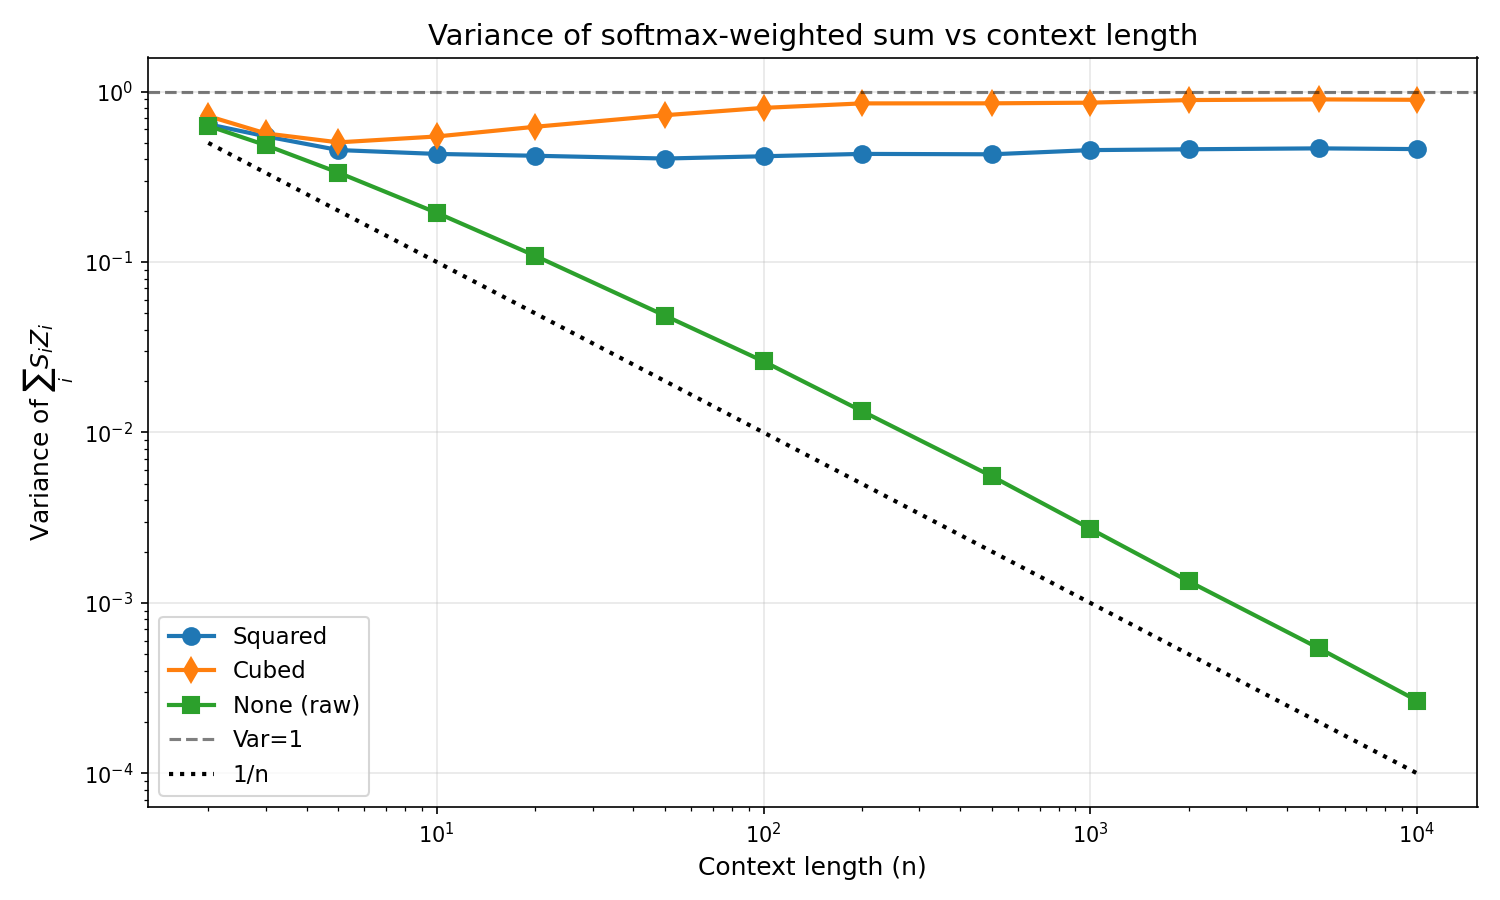
\includegraphics[width=0.72\linewidth]{figures/softmax_weighted_sum_cubed.png}
\caption{Monte Carlo estimate of
$\mathrm{Var}\!\left[\sum_i w_i z_i\right]$ for
$w=\mathrm{softmax}(s^p)$ with Gaussian logits and values, as a function
of context length $n$. Standard attention ($p=1$, ``None'') decays toward
the $1/n$ uniform-attention floor; cubing ($p=3$) drives the variance to 1
(single-token collapse); squaring ($p=2$) is stable between the two for
all $n$ up to $10^4$.}
\label{fig:variance}
\end{figure}

Figure~\ref{fig:variance} confirms this numerically out to $n=10^4$:
$p=1$ decays steadily toward the $1/n$ floor, $p=3$ saturates at 1, and
$p=2$ holds a stable intermediate value across three orders of magnitude
of context length. Squaring is thus not one arbitrary sharpener among
many: among elementwise powers it is \emph{the} critical exponent at which
softmax attention neither washes out nor degenerates as context grows.
Note also that squaring is sign-symmetric: strongly negative logits receive high weight along with strongly positive ones, so the model
must (and, empirically, does) learn score distributions compatible with
this.

We do not claim novelty for logit squaring itself, which we encountered in
an informally circulated article; it belongs to the same family of
length-robust sharpening interventions as Scalable-Softmax
\citep{nakanishi2025scalable} and the temperature adjustments analyzed by
\citet{velickovic2024softmax}. The experimental point here is different
and, to our knowledge, new: sharpening alone rescues nothing: it converts slow decay into flat generalization \emph{only} on top of a
positional scheme that is itself length-stable
(Section~\ref{sec:results}).

\section{Training protocol}
\label{sec:training}

All variants train identically: AdamW ($\beta=(0.9, 0.999)$, weight decay
0.1), learning rate $3\times10^{-4}$ with 500-step linear warmup and
cosine decay, batch size 64, 15{,}000 steps, $\sim$7 minutes per variant
on a single consumer GPU. Loss is cross-entropy on second-occurrence value
digits only.

\paragraph{Context-length curriculum.} Training proceeds at $n=2$ keys
until step 750, $n=4$ until 1{,}500, $n=6$ until 2{,}500, then $n=8$
thereafter. This is not a convenience but a necessity for the
full-attention RoPE variants: trained at $n=8$ from the start, every
variant whose RoPE layers see full attention (\texttt{rope},
\texttt{partial\_rope}, both \texttt{nowindow} hybrids) falls into a
local optimum that predicts values from \emph{positional} statistics
rather than content matching and plateaus at $\sim$37\% exact match
\emph{at the training length}. Started at $n=2$, where only 2 keys exist and no positional shortcut is available, the content-matching
circuit forms first, and every variant then reaches $\approx$100\%
in-distribution accuracy. The windowed hybrids learn the task with or
without the curriculum. This is consistent with reports that length
generalization is sensitive to optimization trajectory rather than
capacity \citep{zhou2024transformers}.

\paragraph{Seeds.} Every variant uses seed 0 except the plain
\texttt{hybrid}, which uses seed 1: at seed 0 it converges to a partial
positional shortcut and plateaus at $\sim$78\% in-distribution retrieval.
Its squared-logit counterpart shows no such sensitivity. We report this
rather than hide it; single-seed results are a stated limitation
(Section~\ref{sec:limitations}).

\section{Results}
\label{sec:results}

\begin{figure}[t]
\centering
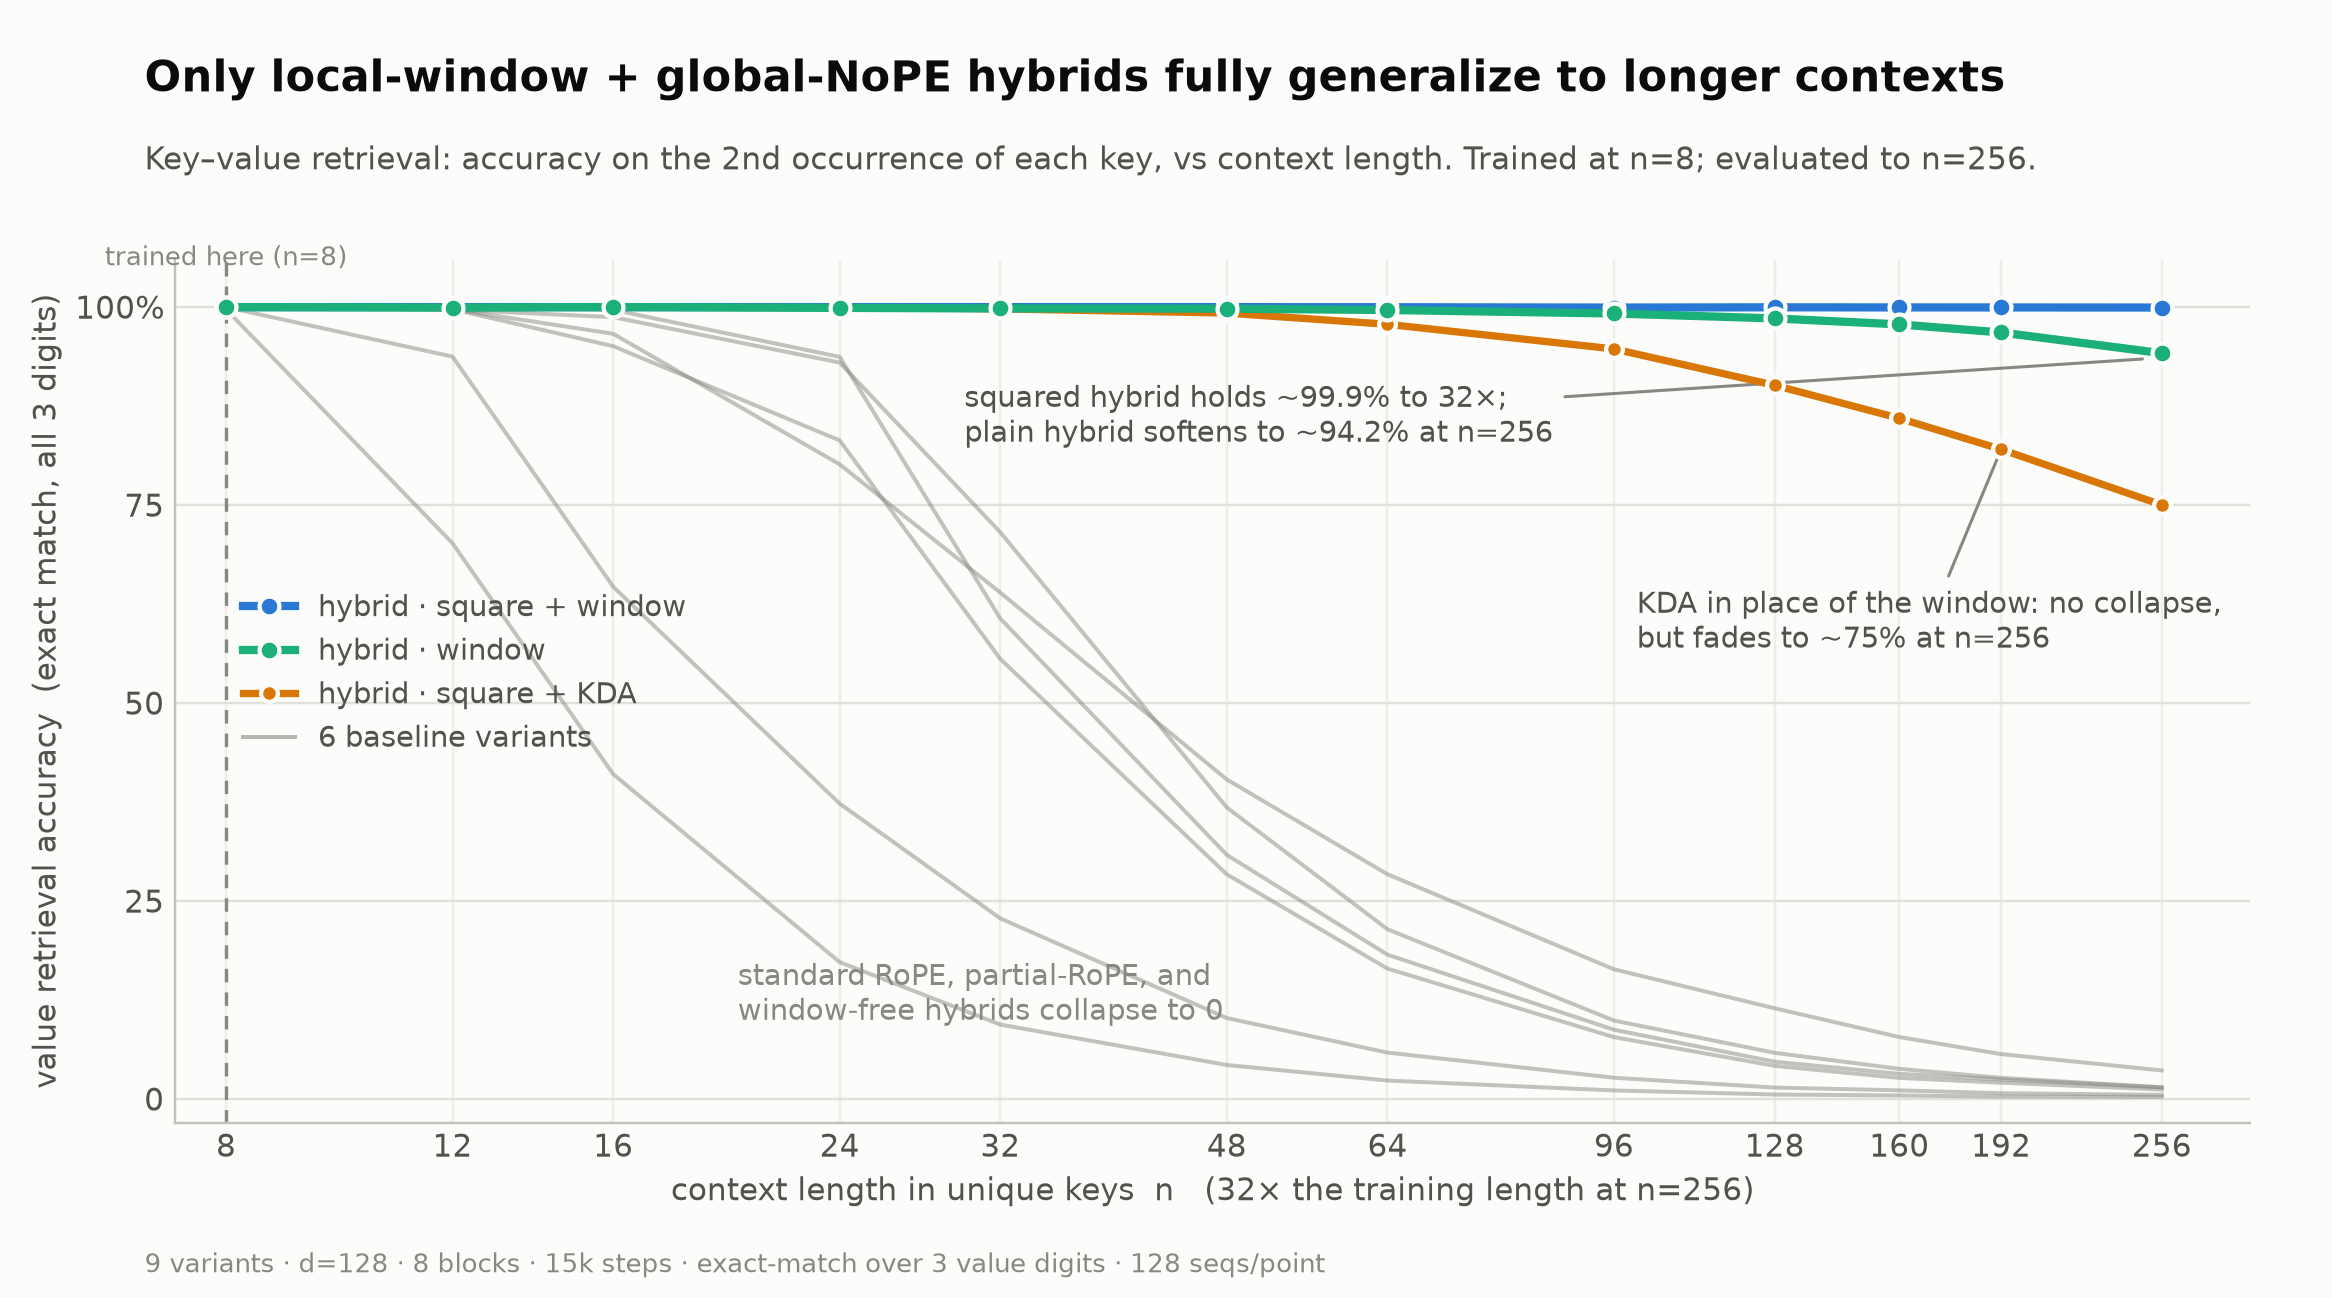
\includegraphics[width=\linewidth]{figures/fig_generalization.png}
\caption{Exact-match retrieval accuracy (all 3 value digits) on second
occurrences versus context length $n$ (unique keys), 128 sequences per
point. All variants are trained at $n=8$ (dashed line) and reach
$\approx$100\% there. Only the windowed interleaved variants generalize:
\texttt{hybrid\_square} holds $\sim$99.9\% to $n=256$ ($32\times$
training length); plain \texttt{hybrid} declines to $\sim$94.2\%. The
KDA variant \texttt{hybrid\_square\_kda} avoids collapse but fades to
$\sim$75\% at $n=256$. All six remaining variants (full RoPE, partial RoPE, and the window-free hybrids, with or without squared logits) collapse toward zero.}
\label{fig:generalization}
\end{figure}

\begin{figure}[t]
\centering
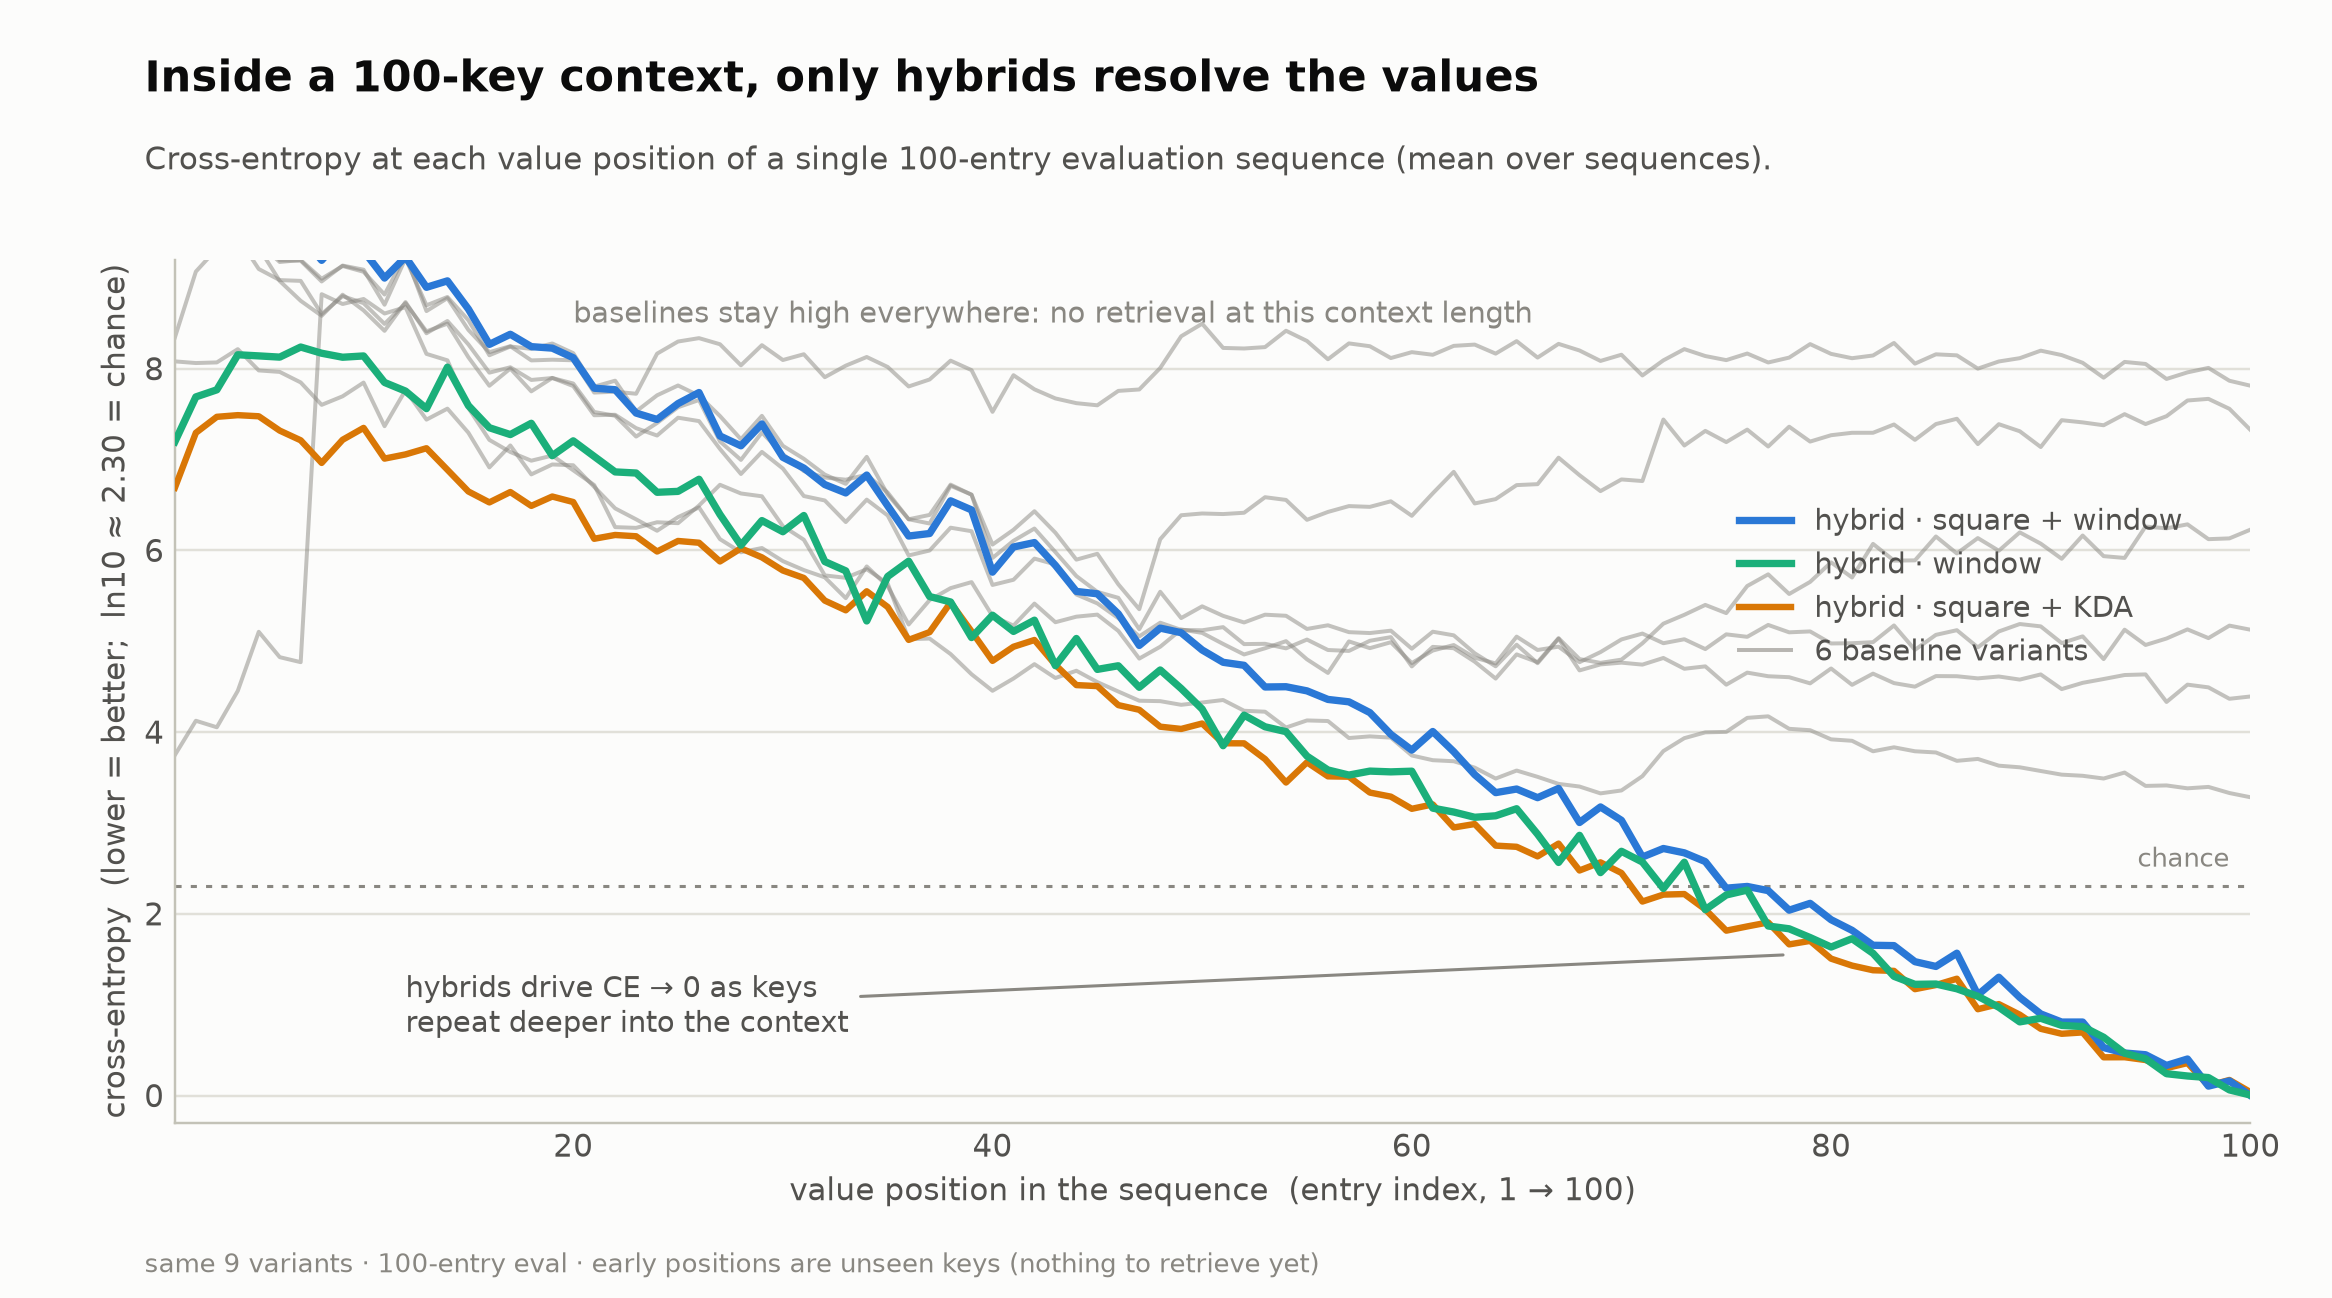
\includegraphics[width=\linewidth]{figures/fig_per_index_ce.png}
\caption{Mean cross-entropy per value digit at each entry index of a
100-entry evaluation sequence ($n=50$ keys, $12.5\times$ training
length). Early entries are mostly first occurrences (nothing to
retrieve), so all models sit above chance ($\ln 10 \approx 2.30$,
dotted); as the sequence progresses, an increasing fraction of entries
are second occurrences. Both windowed hybrids and the KDA hybrid drive
CE toward 0 deep into the context; the six baselines never descend below chance at any position: they perform no retrieval at all at this length.}
\label{fig:perindex}
\end{figure}

\paragraph{In distribution, everything works.} With the curriculum, all
nine variants reach $\approx$99--100\% exact-match retrieval at the
training length $n=8$. Whatever separates the variants, it is not the
ability to learn the task.

\paragraph{Out of distribution, the factorial structure is stark
(Figure~\ref{fig:generalization}).} The two windowed interleaved variants
are the only survivors. \texttt{hybrid\_square} is essentially flat:
$\sim$99.9\% at $n=256$, i.e.\ retrieval is unimpaired at $32\times$ the
training context. Plain \texttt{hybrid} decays gently ($\sim$94\% at $n=256$): the diffusion effect of Section~\ref{sec:square} at work on
an otherwise sound positional scheme. Every other variant collapses:
full RoPE and partial RoPE fail because unseen relative distances place
their attention out of distribution
\citep{su2021roformer,press2021train,kazemnejad2023impact}, and squaring does not save them: sharpened attention to the wrong places is still
wrong. Most diagnostically, \texttt{hybrid\_nowindow} and
\texttt{hybrid\_square\_nowindow} also collapse, no better than plain
RoPE: interleaving NoPE layers is not enough. If even alternate layers
apply RoPE over unbounded distances, the stack inherits RoPE's failure;
the sliding window is what keeps every rotary comparison inside the
training distribution.

\paragraph{KDA: no collapse, graceful fade.} The ninth variant sits in a
class of its own. \texttt{hybrid\_square\_kda} is the only variant
without a sliding window that does not collapse: retrieval is perfect
through $n=24$, $\sim$99.8\% at $n=32$, then fades smoothly: 97.8\% at
$n=64$, 90.1\% at $n=128$, 75.0\% at $n=256$. Its per-position
cross-entropy at the 100-entry evaluation length is indistinguishable
from the windowed hybrids' (Figure~\ref{fig:perindex}), so the shortfall
is purely a long-context effect, not weaker retrieval. The comparison
localizes what the window contributes: a $W=10$ window computes the
\emph{identical} function at every context length, whereas KDA is only
approximately local. Its decay gates are trained on 128-token sequences,
and whatever state survives longer horizons than training presents is a
distribution shift the downstream NoPE retrieval layers never saw; its
fixed-size state must also compress an ever-longer past. The result
supports a refinement of our main claim: a fading local memory
interleaved with NoPE globals suffices to \emph{avoid collapse}, but the
window's exact, structural locality is what converts graceful
degradation into flat generalization.

\paragraph{Per-position behavior (Figure~\ref{fig:perindex}).} Within a
100-entry sequence ($12.5\times$ training length), both windowed hybrids
drive cross-entropy toward zero as keys begin to repeat deeper in the
context, while all six baselines remain \emph{above} chance at every position: at this length they are not degraded retrievers but
non-retrievers. The hybrids' early-position CE is above the baselines'
(the cost of having no global position signal when nothing is yet
retrievable), a price paid exactly where it does not matter.

\section{Related work}

\textbf{Positional encodings and length generalization.} RoPE
\citep{su2021roformer} does not extrapolate; ALiBi \citep{press2021train}
attacked train-short/test-long directly via linear distance penalties
(a soft locality bias related in spirit to our hard window);
interpolation and frequency-scaling methods
\citep{chen2023extending,peng2023yarn} patch RoPE post hoc.
\citet{kazemnejad2023impact} showed NoPE decoders length-generalize
better than explicit encodings on synthetic tasks, and
\citet{wang2024length} extended the case for position-free causal
attention. Our contribution to this line is the controlled factorial
finding that NoPE layers generalize retrieval \emph{only} when the
accompanying RoPE layers are windowed.

\textbf{Interleaved local/global attention in production models.}
Sliding-window attention appeared in Mistral \citep{jiang2023mistral};
Gemma~2 \citep{gemmateam2024gemma2} interleaves local and global RoPE
layers; Llama~4 \citep{meta2025llama4} interleaves windowed-RoPE layers
with position-free global layers (``iRoPE'') explicitly for long-context
generalization. Our windowed hybrid is a minimal instance of this design,
and our ablations isolate \emph{which} ingredient carries the
generalization (the window on rotary layers, with NoPE globals doing the
lookup) at a scale where every alternative can be trained and compared
exactly.

\textbf{Linear attention and delta rules.} Delta-rule fast weight
programmers \citep{schlag2021linear} replace softmax attention with a
recurrent associative memory; Gated DeltaNet \citep{yang2024gated} adds
a per-head forget gate, and Kimi Delta Attention
\citep{kimiteam2025linear} refines the gate to be channel-wise. Kimi
Linear and Kimi K3 \citep{kimiteam2026k3} interleave KDA with NoPE
global attention (3:1 with gated MLA in K3): structurally the same
recipe as our windowed hybrid, with the window replaced by a learned
fading memory. Our controlled substitution (Section~\ref{sec:results})
shows the two are not equivalent under train-short/test-long: KDA
preserves the non-collapse property of the recipe but trades the
window's exact length-invariance for smooth degradation.

\textbf{Attention dispersion and sharpening.}
\citet{velickovic2024softmax} prove softmax attention must disperse as
input length grows and propose temperature adaptation;
Scalable-Softmax \citep{nakanishi2025scalable} rescales logits with
$\log n$. Elementwise squaring is a fixed, length-independent
alternative sitting at the critical exponent of
Section~\ref{sec:square}. Our results position sharpening as a
\emph{second-order} correction: necessary for flat (rather than slowly
decaying) retrieval, sufficient for nothing on its own.

\textbf{Retrieval benchmarks and mechanisms.} Our task distills the
key--value retrieval components of RULER \citep{hsieh2024ruler} and
needle-in-a-haystack tests \citep{kamradt2023needle} into a minimal,
chance-calibrated form, and the underlying circuit is induction-head-like
content matching \citep{olsson2022context}. Sensitivity of length
generalization to optimization details echoes
\citet{zhou2024transformers} and \citet{anil2022exploring}.

\section{Limitations}
\label{sec:limitations}

These results are an existence proof and failure catalogue at small
scale, not a demonstration at LLM scale. Specifically: (i) models are
$\sim$2.1M parameters on a 12-token vocabulary; whether the factorial
pattern survives natural language pretraining at scale is untested here,
though the convergent design of production models
\citep{gemmateam2024gemma2,meta2025llama4} is encouraging. (ii) Each
variant is a single training run; we directly observed seed sensitivity
in one variant (\texttt{hybrid}, seed 0 vs.\ 1), so per-variant accuracy
numbers carry run-to-run uncertainty that we have not quantified with
multi-seed error bars. (iii) The task has exact 3-token key matches;
fuzzy or semantic retrieval may load differently on positional
information. (iv) The variance analysis of Section~\ref{sec:square}
assumes i.i.d.\ Gaussian logits independent of values, a caricature of trained attention; we offer it as an explanation of the observed
stability, not a theorem about trained networks. (v) Squared logits make
attention sign-symmetric, and their interaction with language modeling
objectives (as opposed to pure retrieval) is unexplored here. (vi) The
KDA comparison inherits these caveats and adds its own: it is a single
run at head dimension 32 (K3 uses 128), we did not tune $g_{\min}$, the
KDA:global ratio (1:1 here versus K3's 3:1), or the training length its
decay gates adapt to, and any of these could narrow the gap to the
window.

\section{Conclusion}

On a minimal key--value retrieval task, we trained eight attention
variants differing only in positional treatment and logit sharpening,
and found a sharp factorial answer to context-length generalization:
confine rotary position encodings to a short sliding window, let
interleaved position-free layers do global content lookup, and square the attention logits; retrieval is then essentially perfect at $32\times$
the training length, while every ablation of the positional recipe
collapses to zero. The window is load-bearing, sharpening is a
second-order stabilizer with a principled critical exponent, and a
context-length curriculum decides whether full-attention RoPE models
learn retrieval at all. A ninth variant substituting Kimi K3's delta-rule
linear attention for the sliding window shows the recipe's local
component can be learned rather than structural, at the price of smooth
degradation ($\sim$75\% at $32\times$) in place of flat generalization. We release the benchmark, all specs, and training
code at \href{https://github.com/6elphegor/kvbench}{\texttt{github.com/6elphegor/kvbench}};
each variant trains in minutes on one consumer GPU, making this an easy
substrate for testing further attention designs.

\section*{Acknowledgments}

The manuscript and the benchmark implementation were drafted with the
assistance of Claude (Anthropic). The research questions, experimental
design, and interpretation of results are the author's, who takes full
responsibility for all content.

\bibliographystyle{plainnat}
\bibliography{references}

\end{document}
